\documentclass{article}
\usepackage[spanish]{babel}
\usepackage{graphicx}
\usepackage{xcolor}
\usepackage[utf8]{inputenc}
\usepackage{fancyhdr}
\usepackage{lastpage}
\usepackage{enumitem}
\usepackage{listings}
\usepackage{verbatim}
\usepackage{float}

\pagestyle{fancy}
\fancyhf{}
\rfoot{Page \thepage\hspace{1pt} de~\pageref{LastPage}}

\title{Tarea de errores de seguridad en Administración de Base de Datos}
\author{
Guillermo López García
\and
Adrián Dávila Guerra
}

\begin{document}
\maketitle

\begin{enumerate}[label=\alph*]
    \item \textbf{1º Parte. ¿Qué ocurrió?}\\
        Ocurrió una brecha de seguridad en las base de datos de los Hoteles Marriott.
    En este caso, sucedió que se hubo un acceso indebido directamente a la base
    de datos, en concreto a la parte que se encargaba de almacenar el
    sistema de fidelidad Starwood (adquirido poco antes por la cadena de hoteles
    comprando a la empresa que lo desarrollo). Los datos que se obtuvieron tenían
    que ver con la reserva y compra de los servicios desde el año 2014 hasta
    el 10 septiembre de 2018. Dichos datos, iban desde un simple nombre
    hasta los datos cifrados de las cuentas bancarias.\\
    El único problema, es que para descrifrar los datos solo hacían
    falta otros dos factores, y es posible que los atacantes ya los
    hubieran obtenido.
    
    \item \textbf{2º Parte. ¿Qué falló?}\\
        El acceso fraudulento se dió debido a que las credenciales de acceso
    al sistema de base de datos estaban relacionadas con la vida personal
    de los propios administradores.\\
    Citando a Bimal Gandhi, director ejecutivo de Uniken:
    `Esta brecha de seguridad subraya la `pura locura'
    de seguir confiando en métodos de seguridad obsoletos, como el uso de
    información personal en la autenticación, dada la gran proliferación
    de datos personales robados y filtrados ahora disponibles en la web
    oscura'. Además, las claves para descifrar los datos sensibles como
    las cuentas bancarias estaba en el mismo sistema vulnerado.\\
    Con lo cual, se dio todas las condiciones para dar en bandeja de plata
    toda la información personal sensible a los atacantes.
    
    \item \textbf{3º Parte. ¿Qué tecnología estaba implicada?}\\
        Estaba implicada tecnología web y sistemas de base de datos.
    Los artículos leidos respecto al tema no dejan claro si es
    una base de datos relacional o NoSQL\@. Respecto a la tecnología
    web de donde pudieron obtener el fallo inicial para posteriormente
    acceder de forma directa, tampoco quiere dar detalles la empresa
    dueña de la cadena de hoteles Marriott.
    
    \item \textbf{4º Parte. ¿Comó se pudo haber solucionado?}\\
        Una de las principales soluciones se podría dar no utilizando
    información personal en la autenticación.
    Gran parte de los usuarios debería haber sido más consciente en no utilizar sus datos
    personales como medio para autentificar en la base de datos de Starwood Hotels,
    por lo que, tanto los usuarios como los propios administradores de la base de datos de
    esta cadena de hoteles se tuvo que tomar medidas para evitar el robo de datos. \\
    Para solucionar este problema debe cumplir lo siguiente:
    
    \begin{itemize}
        \item Los usuarios NO deben añadir una fecha de nacimiento como contraseña, número de teléfono,
              nombre o cualquier dato que se contemple en los datos personales del usuario,
              incluso de otra información no reflejada en los datos personales en otros medios
              como las redes sociales.
        \item Los usuarios DEBEN utilizar una contraseña que use caracteres con mayúsculas,
              minúsculas, campos numéricos y símbolos permitidos y correctos
              (el tipo de formato de codificación de caracteres permitido).
        \item Por otro lado, los administradores de la base de datos deben tener en cuenta los
              riesgos que podría tener el cifrado AES-128.
        \item No sólo importa el cifrado de las contraseñas, sino que también se debe tener en cuenta
              la seguridad del acceso a la base de datos. Por ejemplo, controlar los accesos por IP y ubicación.
    \end{itemize}

    \item \textbf{5º Parte. ¿Dondé ocurrió?} \\
        En la cadena de Hoteles Marriott, surgió a el ataque a partir de la red de Starwood Hotels
        \begin{figure}[H]
        \centering
        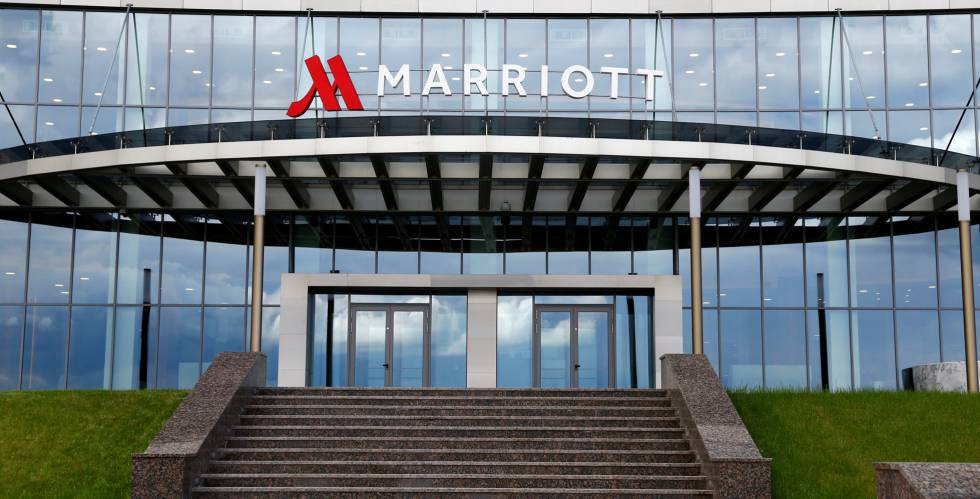
\includegraphics[width=0.7\linewidth]{./marriott}
        \caption{Hoteles Marriott}
        \end{figure}
\end{enumerate}
\end{document}

% Ayuda para crear un buen estilo en la memoria.
%\begin{enumerate}
    %\item \underline{}:
%\end{enumerate}
%\lstset{
  %language=...,
  %texcl=true,
  %basicstyle=\ttfamily,
  %columns=fullflexible,
  %frame=single,
  %breaklines=true,
  %postbreak=\mbox{\textcolor{red}{$\hookrightarrow$}\space},
%}
%\lstinputlisting[]{base_de_datos/sql.sql}
%\begin{figure}[H]
%\centering
%\includegraphics[width=0.7\linewidth]{./...}
%\caption{...}
%\end{figure}

